\chapter{Semana 1: análisis de requisitos y selección del estilo arquitectónico}

Durante la primera semana de la práctica se realizó el análisis de los requisitos funcionales y de dominio del periódico digital y se comenzó a definir su arquitectura software. En esta primera fase se plantearon distintas alternativas para organizar el sistema, comenzando con una propuesta monolítica que posteriormente fue revisada y sustituida por una arquitectura cliente-servidor con API REST.

Las decisiones correspondientes a esta primera semana quedaron estudiadas en las ADR-0001.1, ADR-0001.2 y ADR-0001.3.

\section{Decisión inicial: arquitectura monolítica}

En la primera decisión arquitectónica, \href{Decisiones/0001.1-seleccion-estilo-arquitectonico-global.md}{ADR-0001.1}, los arquitectos senior propusieron una arquitectura monolítica basada en MVC. Esta primera opción permitía organizar la presentación, la lógica de negocio y el acceso a datos dentro de una misma aplicación. Se consideró inicialmente por su sencillez y porque permitía establecer una primera estructura para las funcionalidades del periódico.

Sin embargo, durante la revisión realizada por los arquitectos cognitivos se plantearon dudas sobre la separación entre la interfaz web y la lógica de negocio. Se cuestionó la utilidad de mantener ambas responsabilidades dentro de una misma aplicación, además de la necesidad de diferenciar mejor la parte de presentación de los servicios del backend para organizar las suscripciones, los pagos mediante Stripe y las estadísticas.

A partir de estas observaciones, los arquitectos senior revisaron la propuesta y volvieron a valorar las alternativas arquitectónicas.

\section{Revisión de las alternativas y cambio de arquitectura}

Durante la revisión se consideraron las alternativas recogidas en las decisiones arquitectónicas: una arquitectura monolítica basada en MVC, una arquitectura cliente-servidor con API REST, una arquitectura orientada a servicios (SOA) y una arquitectura de microservicios orientada a eventos.

La propuesta monolítica inicial permitía mantener una estructura sencilla, pero se consideró que una arquitectura cliente-servidor representaba mejor la separación entre el frontend web y el backend que se buscaba para este sistema.

En cuanto a SOA, se descartó porque la incorporación de un bus de servicios y una estructura de integración más amplia añadía demasiada complejidad para lo que se pedía. La alternativa de microservicios también se descartó, ya que suponía dividir el periódico en diferentes servicios independientes y gestionar su comunicación.

Finalmente, se eligió una arquitectura cliente-servidor con API REST. Esta opción permite diferenciar la interfaz utilizada por los lectores de los servicios encargados de gestionar las funcionalidades del periódico y establecer la comunicación HTTP/REST indicada en el requisito RD2.

Tras esta revisión, se documentó la anulación de la propuesta inicial en la \href{Decisiones/0001.2-anulacion-decision-0001.1.md}{ADR-0001.2}. La nueva solución quedó recogida en la \href{Decisiones/0001.3-migracion-estilo-cliente-servidor-api-rest.md}{ADR-0001.3}.

\section{Arquitectura cliente-servidor con API REST}

La arquitectura seleccionada establece una separación entre el frontend web, encargado de la presentación e interacción con los lectores, y el backend, donde se encuentran los servicios relacionados con las noticias, las suscripciones, la facturación y las estadísticas. El frontend debe permitir el acceso desde PC y Tablet, mientras que el backend se encarga de procesar las peticiones y gestionar las operaciones del sistema. La comunicación entre ambas partes se realiza mediante HTTP/REST, como se establece en el requisito RD2.

\section{Representación de la arquitectura en UML}

Según la primera propuesta, los arquitectos junior elaboraron un diagrama UML basado en la arquitectura monolítica.

\begin{figure}[H]
    \centering
    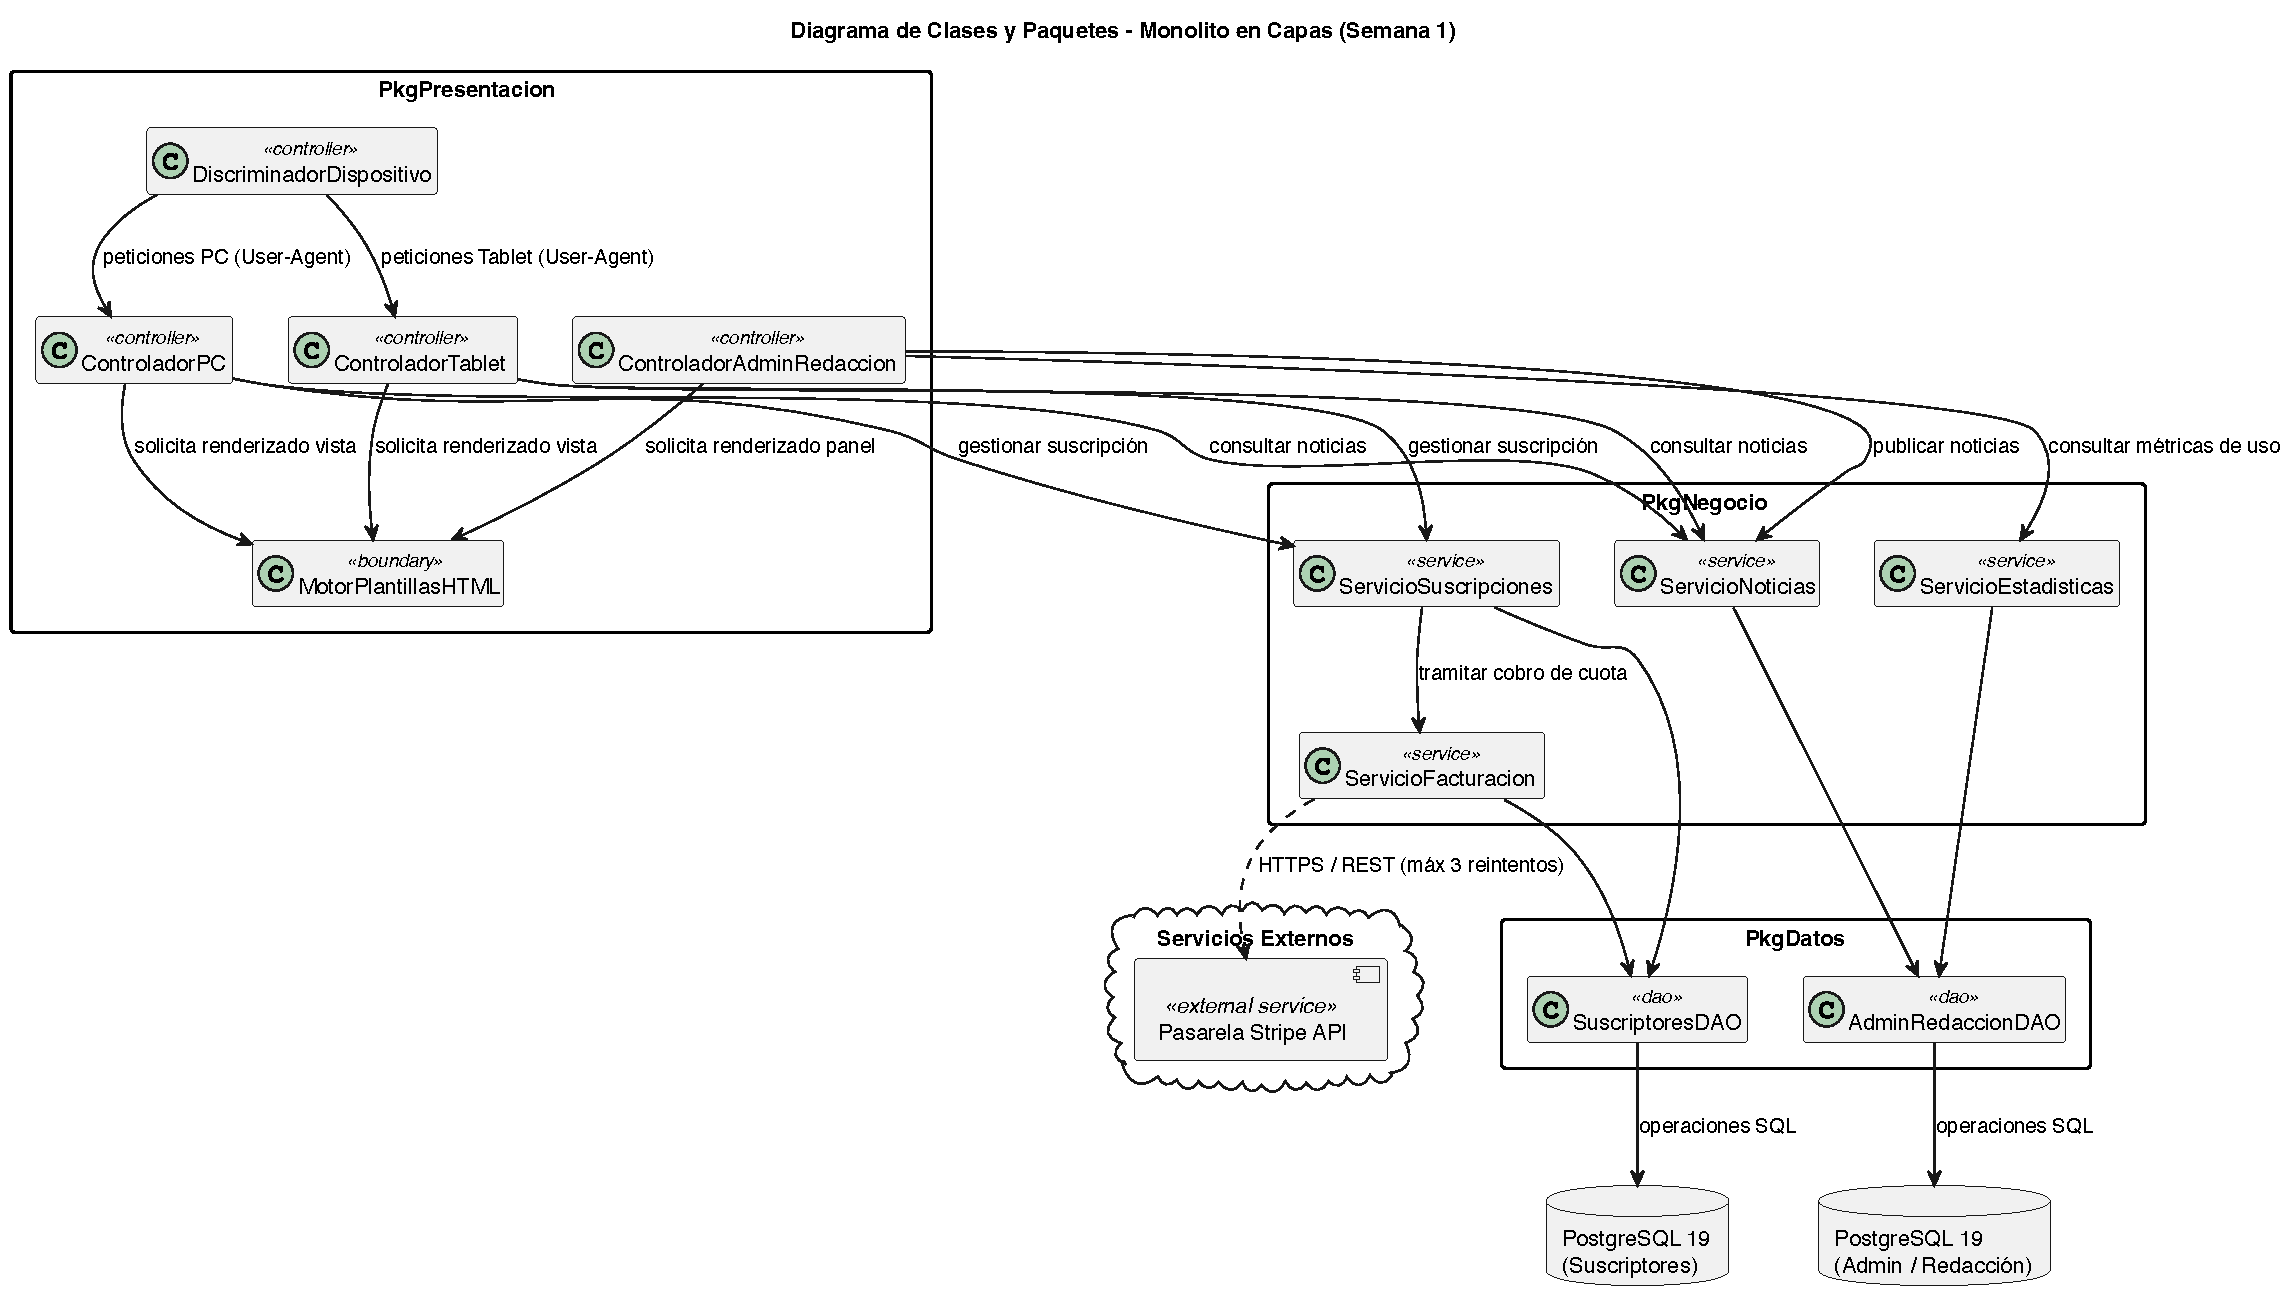
\includegraphics[width=0.9\textwidth]{assets/0001-estilo-arquitectonico-monolito-semana1.pdf}
    \caption{Primera propuesta de arquitectura monolítica.}
    \label{fig:arquitectura-monolitica}
\end{figure}

Durante la revisión del diagrama se encontraron algunos aspectos que debían corregirse. El primero estaba relacionado con la organización general del sistema. El diagrama representaba la propuesta monolítica inicial, que posteriormente fue anulada tras la discusión entre los arquitectos senior y cognitivos. Además, en esta primera representación se había incorporado un componente de base de datos antes de haber definido cómo debía organizarse el acceso a los datos.

En esta primera fase el objetivo era definir el estilo arquitectónico, por lo que todavía no era necesario entrar en tanto detalle sobre las bases de datos. Esto no significa que no deban aparecer en la arquitectura, ya que se exigen dos bases de datos PostgreSQL 19: una para administradores y redactores y otra para suscriptores.

Por tanto, el primer UML se mantiene como parte de la evolución del proyecto, aunque no representa la arquitectura finalmente seleccionada. La revisión permitió comprobar la importancia de que los componentes y las relaciones del diagrama se correspondan con las decisiones arquitectónicas tomadas.

\section{Resultado de la primera semana}

La primera semana finalizó con el análisis de requisitos mejorado y simplificado, ciñéndose a lo solicitado, y la elección de una arquitectura cliente-servidor con API REST. La propuesta monolítica inicial fue anulada después de las observaciones realizadas por los arquitectos cognitivos y de la comparación con otras alternativas. Las decisiones ADR-0001.1, ADR-0001.2 y ADR-0001.3 recogen la evolución de este primer problema de diseño.

La representación UML inicial también permitió detectar aspectos que debían revisarse antes de continuar desarrollando las clases y paquetes del sistema.
